% Template for BJ paper in LaTeX (Jan Hrabe, NKI, 05/16/2005)
%
% To compile into a document, run
% latex bj_latex_template
% bibtex bj_latex_template
% latex bj_latex_template (run 2-3 times repeatedly)
% dvips bj_latex_template.dvi
%
% or replace the latex command by the pdflatex command in the lines above to
% generate a PDF file and use acroread or xpdf for viewing and
% printing instead of the postscript generating program dvips

% Use standard article document class with slightly bigger font and 
% a separate title page
%\documentclass[11pt,titlepage]{article}
\documentclass[12pt,letterpage]{article}
\usepackage{graphics,tabularx,subfigure,color,calc,verbatim,epsfig,fullpage,authblk,appendix}
\usepackage[normalem]{ulem}
%\usepackage{wrapfig}

% Packages to load (all standard on a modern LaTeX system on Linux)

% Make doublespaced ugly typography required for mysterious 
% reasons by most journals - comment out for normal output
\usepackage{setspace} 
%\doublespacing

% AMS-Math package to have nice multi-line equations and other goodies
\usepackage{amsmath}

% Show labels for easy orientation, comment out for final version
% \usepackage{showlabels}

% EPS/PDF graphics
% Place figures in the document directory in both the EPS and PDF
% formats, e.g., fig_1.eps and fig_1.pdf. Use the includegraphics
% command without file extension, e.g. \includegraphics*[width=3.25in]{fig_1}
% The pdflatex or latex programs then work automagically with the 
% appropriate formats.  EPS figures can be converted to PDF using
% the epstopdf program present on most Linux disributions
\usepackage{graphicx}
\usepackage{tikz}
\usetikzlibrary{arrows,chains,matrix,positioning,scopes}
% Following packages are used to include hyper link in file.
\usepackage{xcolor}
\usepackage[colorlinks,
            linkcolor=blue,
            anchorcolor=green,
            citecolor=purple]{hyperref}
\usepackage{threeparttable}
\usepackage{listings}
% Citation style in the text: numbers in parenthesis, sorted by their
% order in the list of references.
% Uses a range if possible: (1-3), not (1,2,3)
\usepackage[round,numbers,sort&compress]{natbib} 
\setlength{\textwidth}{6.5in}
\setlength{\textheight}{20.5cm}
\setlength{\oddsidemargin}{0.0cm}
\setlength{\topmargin}{0 cm}

% Numbering style in the list of references: a number followed by a period
%\renewcommand{\bibnumfmt}[1]{#1.}
\makeatletter
\renewcommand\@biblabel[1]{#1.}
\makeatother

\makeatletter
\def\@cite#1#2{$()#1\if@tempswa , #2\fi$}
\makeatother
% Examples of special definitions (amsmath package required)
\newcommand{\erf}{\operatorname{erf}}        % error function
\newcommand{\erfc}{\operatorname{erfc}}      % complementary error function
\newcommand{\BibTeX}{\textsc{Bib}\TeX}       % corect BibTeX appearance

\def\chapdir{chapter}
\def\bibstldir{.}
\def\bibdir{.}

\title{Molecular Dynamics Investigation of the Compression and Shearing of Polymer Nano-Composite Systems}

\iffalse 
\author{Lei~Wang\thanks{
           Haojun Liang.  Address:
           Polymer Science and Engineering,
	       Department of Chemistry, ,
	   Hefei, Anhui~230026, P.R.China,
	   Tel.:~(+86)551-3600240, Fax:~(+86)000-0000} \\
	Department of Chemistry, \\
	University of Science and Technology of China, Hefei, Anhui 
	\and Xueqing Zou \\
	Department of Biology, \\
	Beckmann Institute, Urbana, Illinois}

% Revision date - uncomment to exclude date in the final version
%\date{}

% Running head
\pagestyle{myheadings}
\markright{Short paper title}
\fi

\author[$^{\dag}$]{Ningning Lin}
\author[$^{\dag}$]{Wang Lei}
\author[$^{\dag}$]{Yuan Liu}
\author[,$^{\dag}$]{Haojun Lian \footnote{To whom correspondence should be addressed. E-mail: hjliang@ustc.edu.cn; Phone: +86-551-3607824; Fax: +86-551-3607824}}

\affil[$^{\dag}$]{University of Science and Technology of China, Hefei, Anhui, China}
%\affil[$^{\S}$]{Applied Physics and Center for NanoScience, Ludwig-Maximilians-Universit\"{a}t M\"{u}nchen, Munich, Germany}
%\affil[$^{\P}$]{Department of Mathematics, University of Illinois, Urbana, Illinois, USA}

% We are done with the headers, the actual document starts here
\begin{document}
%\singlespace
% generate the title page from the info in the headers above
\maketitle

% 200 words max Abstract
\abstract{
 Using molecular dynamics soft package LAMMPS, we investiage the procedures of compression and shearing of Polymer Nano-sized-fillers Composits (PNCs) based on well parameterized coarsed-grained model. The addition of the nano-sized fillers to the polymer matrix reinforced the mechanical properies of the system. Interestingly, at above or beneath the glass transition temperature, it behaves independent responses to the coppression or the shearing, and the mechanism behind these phenomena are different. The further analysis of Radius Distribution Function (RDF), and the change of the contacting number between polymer and filler, suggest that the reinforcement of the mechanical properties depends on various factors, such as the size and the shape of the filler, the strength of the interaction between polymer and filler, and etc.. 
}

% New page
\clearpage

\section*{Introduction}
From long ago till recently, people are devoted to the discuttion and investigation of improving the performances of polymer product to meet their different desire. By adding nano- or micro-sized fillers to the polymer matrix, we found thus we are able to change the polymers' mechanical, optical, chemical or electrical properties.~\cite{Kutvonen2012,Humphrey1996a,Plimpton1995,Yoon2002,Chapman2001,Schmidt2003} But the mechanism of the reinforcement of the Polymer Nano-sized-filler Composite (PNC) are still elusive. It is widely acknowledged that there are many influencing factors to this matter, such as, the shape and the size of the filler, the molecular weight of the polymer, the degree of crosslinking of the polymer matrix, the strength of the interaction between the polymer and the filler, the mass-loading of the filler, and dispersity of the filler in the polymer matrix. As the development of the Nano-technology, we already get some advance from both experimental and theoretical points of view, however, the response of NPC to the compression and the shearing, and the mechanism behind are not very well studied and need more profound insigts. 

We now are able to use computer simulation to study PNC systems at the atom scale in detail, taking advantage of fast growth of the computer science and technology. Dilip Gersappe depicted a Coarse-Grained (CG) Model of PNC system in 2002, and investiaged the PNC system responses to the tensile~\cite{Gersappe2002}. Aki Kutvonen and etc. then studied the tensile of the PNC system using a CG model, and demonstrated that the size, the shape, the mass loading and the surface area of the filler will affect the properties of the PNC system.~\cite{Kutvonen2012,Kutvonen2012a} Many other models are then been designed in different scales trying to simulate the tensile, the compression of the PNC systems, and to analyze the inflences of the dispersity of the filler, the strength of the interaction between the polymer and the filler, and other factores, to the properties and the performances of the PNC system.~\cite{Gersappe2002,Liu2011a,Allegra2008,Brown2008,Brown2003} 

Experimental and theoretical models are developed fast and have been studied widely, however, the compression and the shearing of the PNC system are seldomly investigated and the mechanism is still under consideration. We thus simulate the compression procedure of the PNC system, using a CG model built and manipulatd by the molecular dymamics soft package LAMMPS~\cite{Wu2011}, to investigate the response of PNC to the compression, and describe the mechainism of the reinforcement by the filler to the system. All our analysis of the result are with the help of the software Visual Molecular Dynamics (VMD)~\cite{Hussain2006} 

\iffalse
Citations are made using the \emph{citep} command, e.g., one paper
\citep{el-Kareh_etal93} or more papers
\citep{el-Kareh_etal93,Chen_Nicholson00}.  It works fine with a single
author, two authors, or more.  Books are cited in the same way
\citep{Callaghan91}, book chapters as well \citep{Stiles_Bartol01},
including a chapter in press \citep{Stiles_etal04}.  Abstracts can be
handled too \citep{Tao_etal02}.  Pages can be included in a citation
\citep[pp.~12--18]{Callaghan91}.  Citations in a text form (i.e., author 
name followed by the usual reference number in parenthesis) can be 
done using the \emph{citet} command, e.g., ``an approach used 
by \citet{el-Kareh_etal93}''.
\fi
\clearpage

\section*{Theory}
\input{\chapdir/theory}
\iffalse
Text can reference Eq.~\ref{eqn:symmetry}
\begin{equation} \label{eqn:symmetry}
   \Phi(\vec{r}) = \Phi(-\vec{r})
\end{equation}
anywhere, as long as it is numbered.
\fi
\clearpage

\section*{Methods}


We build up a coarse-grained molecular dynamics model to simulate the NPC systems with LAMMPS, get the trajectory of each production run, then analyze the result using VMD.

\subsection*{The Coarse-Grained Model}
\begin{figure}[h!]
\begin{center}
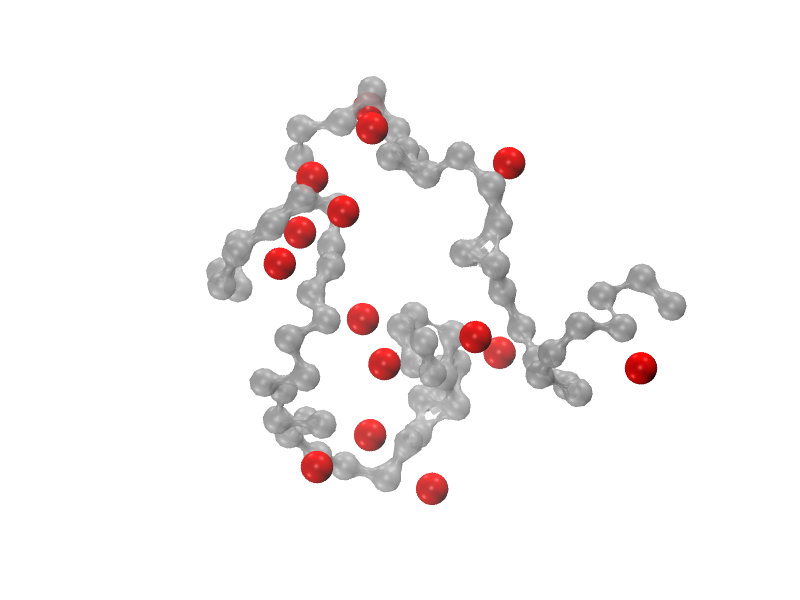
\includegraphics[width=5in]{./figure/pnp.png}
\caption{A snapshot of the CG PNC system, taken with VMD.~\cite{Humphrey1996a}}
\label{fig:pnp_snapshot}
\end{center}
\end{figure}
Using Self-Avoid Walking (SAW) method, we firstly put $N$ polymer chains into a cubic Periodic Boundary Condition (PBC) box. There are $L$ monomers in each chain, and the mass of each monomer is $56$ representing a sum of $4$ carbon and $8$ hydrogen atoms. All bond lengths are set to $4.7~\AA$. Then we put $M$ fillers into the system randomly.~\ref{fig:pnp_snapshot}

The force field we use in our model is simply the Lennard-Jones potential (L-J potential) {eq.~\ref{eq:lj}}, we modify it according to our desire to the L-J potential with radii cut at some certain distance (eq.~\ref{eq:lj_cut}).

\begin{equation}\label{eq:lj}
p^{LJ}(r_{i,j})=4\epsilon_{i,j}\left[ \left(\frac{\sigma_{i,j}}{r_{i,j}}\right)^{12}-\left(\frac{\sigma_{i,j}}{r_{i,j}}\right)^6 \right]
\end{equation}

\begin{equation}\label{eq:lj_cut}
p(r_{i,j})=
\left\{
\begin{array} {l l}
p^{LJ}(r_{i,j}) - p^{LJ}(r_{c}) & \quad (r_{i,j}<r_{c}) \\
0 & \quad (r_{i,j} \geq r_{c})
\end{array} 
\right.
\end{equation}

$\epsilon_{i,j}$ and $\sigma_{i,j}$ are respectively the strength of the interaction, and the equilibration distance of the interacting atom-pair $i, j$ under consideration.

\subsection*{Protocols of Molecular Dynamics Simulation}
After all chains and fillers are positioned in our PBC box, the PNC system is minimized using ${NVE}$ with a limitation imposed on the distance that atoms are allowed to move in one timestep, in our system, $0.05\AA/fs^{-1}$. When the energy of the system reaches the minimum, we compress the system and equilibrate it at $1000K$ (which is adjustable), and then lower it stepwise by the decrement of $50K$, to our desired temperture $T_{eq}$ (i.e., $200K$ in our compression simulation, and $600K$ in the shearing one), the whole procedure is performed using ${NVT}$ updates by far. Equilibrated under $T_{eq}$, the system is then relaxed using ${NPT}$ updates to the pressure $P_{eq}$. The system is ready for any molecular dynamics production run.

\subsubsection*{The Tensiling}
$1.1\times10^{-5}\AA/fs$

\subsubsection*{The Compression}
During the compression procedure, we use the so-called $NL_x\sigma_y\sigma_z T$ ensemble, under which we compress the system along the $X$-axis, and keep the pressure on other directions unchanged at $T_{eq}$. The rate of the compression is $1.0\times10^{-11}\AA/fs$.

\subsubsection*{The Shearing}

\subsection*{Setup of the Systems}
Here is the list of the potential parameters in each system (the substripts $p$ and $f$ represents polymer and filler respectively, the energy unit is $KCal/mol$ and the length unit is $\AA$):
\begin{table}[h!]
\begin{center}
\vspace*{0.5cm}
\begin{threeparttable}
\begin{tabular}{lcccccc}
\hline
Simulation & System & $\epsilon_{p,p}$ & $\sigma_{p,p}$ & $\epsilon_{p,f}$\tnote{*} & $\sigma_{p,f}$\tnote{\dag}\\
\hline
S1 & Polymer     & $1.13$         & $4.7$ &    -    & -     \\
S2 & Polymer-LF  & $1.13$         & $4.7$ & $4.52$  & $9.2$ \\
S3 & Polymer-MF  & $1.13$\tnote{*}& $4.7$ & $4.52$  & $6.1$ \\
S4 & Polymer-SF  & $1.13$         & $4.7$ & $4.52$  & $4.6$ \\
\hline
\end{tabular}
\begin{tablenotes}
\item[*] \small{we keep $\sigma_{f,f}=0.25\sigma_{p,p}$ for all systems.}
\item[\dag] \small{Except $r_{cp,f}=2.1\sigma$, $r_{c}=2.1\sigma$ for all $i,j$ atom-pairs}
\end{tablenotes}
\end{threeparttable}
\caption{List of simulations}
\label{simu_summary}
\end{center}
\end{table}
\iffalse
我们初步建立了四类体系,各体系里包含128条含有64个粗粒化单元的高分子链和不同的纳米颗粒(表1)。
表 1 体系参数
2. 力场
	我们将Dilip Gersappe研究PNC拉伸屈服机理[6]提出的模型进行了改进,参数则采用了Aki Kutvone 等人研究复合材料拉伸[8]时的设置。
高分子键 如公式1,在高分子链上两个相邻成键的粗粒化单元间,采用2-4谐振子势。本模型中没有设置高分子链的键角及二面角作用势。
    ,                   (1)
非键作用势 体系内非键连的粒子间都为LJ作用势,如公式2所示。对于高分子粗粒化单元间相互作用,σ=σext,ε=εext 。对于纳米颗粒间的相互作用,εnp=0.25εext ,σ的值为各体系中纳米颗粒的直径σL、σM、σS 。对于纳米颗粒与高分子单元间的相互作用,εpnp=4εext ,σ=(σext+σnp)/2。同一高分子链内的两个非键粗粒化单元间相互作用,截断半径为2^(1/6)σ,其余非键作用的粗粒化粒子截断半径均为2.1σ。具体参数见表2。
 ,                                 (2)
表 2  力场参数
kh	rh0	εext	σext	σS	σM	σL
11.62	4.7	1.13	4.7	4.6	6.1	9.2
注:上图中能量单位为kcal,长度单位为Å

3.模拟过程
	\fi
\clearpage

\section*{Results}
\input{\chapdir/results}
\clearpage

\section*{Discussion}
\subsection*{The Glass Transition Temperature of PNC}
The Glass Transition Temperature of the system considered is expected before hand, since we want to have our result comparable with experiments and the real physical phenomenon.

\clearpage

\begin{appendix}
%\chapter{appendix1}
\input{\chapdir/appendix}
\clearpage
%\chapter{app2}
\end{appendix}

%%%%%%%%%%%%%%%%%%%%%%%
% Figure legends
\iffalse
\section{Figure Legends}
\subsubsection{no Figure}%~\ref{fig:result_fig}.}
Figure legend here.
% Figures, one per page (fig_1.eps and fig_1.pdf files must be present
% in the document directory)

\begin{figure}
   \begin{center}
      \includegraphics*[width=3.25in]{fig_1}
      \caption{}
      \label{fig:result_fig}
   \end{center}
\end{figure}

\clearpage

\fi


\newpage
%%%%%%%%%%%%%%%%%%%%%%%
%\section*{Supplementary Material}
%\input{supp}


\newpage
%%%%%%%%%%%%%%%%%%%%%%%
%\section*{Reply to the Referee}
%\input{Reply}
% Compile and format the bibliography (bj_bibtex_template.bib BibTeX
% file must be present in the document directory)

%%%%%%%%%%%%%%%%%%%%%%%
% Bibliography style (requires the style file biophysj.bst in the 
% document directory)
\bibliographystyle{\bibstldir/biophysj}
\bibliography{\bibdir/pnc}


% closing statement, nothing below matters
\end{document}
